\documentclass[b5paper,10pt]{article}
\usepackage[british]{babel}
\usepackage[top=1.9cm,bottom=1.9cm,left=1.9cm,right=1.9cm]{geometry}
\usepackage{graphicx}
\usepackage{subcaption}
\usepackage[hyphens]{url}
\usepackage{paralist}
\usepackage{authblk}
\usepackage{siunitx}
\usepackage{fancyhdr}
\usepackage[noadjust]{cite}
\usepackage[semicolon,sort&compress]{natbib}
\usepackage[pdftex,breaklinks,colorlinks=true]{hyperref}

\pagestyle{fancy}
\lhead{{\emph{Journal of Urban Technology}}}
\rhead{Electric Vehicle Mobility as-a-Service}

% correct bad hyphenation here
%\hyphenation{op-tical net-works semi-conduc-tor}

% title
\title{Electric Vehicle Mobility as-a-Service: Exploring the
  `Tri-Opt' of Novel Private Transport Business Models}

% names
\author[1]{Peter Cooper}
\author[2]{Theo Tryfonas\thanks{Corresponding author: Theo
                         Tryfonas, Faculty of Engineering, University
                         of Bristol, Queen's Building, University Walk, Bristol BS8 1TR, UK. E-mail: \url{theo.tryfonas@bristol.ac.uk}}}
\author[3]{Tom Crick}
\author[4]{Alex Marsh}
% affiliation
\affil[1]{Faculty of Engineering, University of Bristol, UK}
\affil[2]{Faculty of Engineering, University of Bristol, UK}
\affil[3]{Department of Computer Science, Swansea University, UK}
\affil[4]{School for Policy Studies, University of Bristol, UK}
% emails
\affil[1]{\protect\url{peter.cooper@bristol.ac.uk}}
\affil[2]{\protect\url{theo.tryfonas@bristol.ac.uk}}
\affil[3]{\protect\url{thomas.crick@swansea.ac.uk}}
\affil[4]{\protect\url{alex.marsh@bristol.ac.uk}}

\renewcommand\Authands{ and }
\def\UrlBreaks{\do\/\do-}

\date{ }

\begin{document}
\maketitle

% Submitted abstract, max 200 words on the system:
% Three distinct trends have emerged that have disrupted the dominance
% of privately-owned, combustion car transport in the UK. First, the
% emergence of the electric powertrain as an affordable means of
% transport; the second is the rise of new hire models of car ownership:
% thirdly, the rise of `smart city thinking', the concept that increased
% connectivity and data availability can be harnessed to create value,
% specifically here as it impacts transport. We define the combination
% of the three as the `tri-opt' of private transport -- three disruptors
% that should not be considered in isolation but as interacting levers
% -- an inflection of the `Energy Trilemma'.

% In this paper, we apply systems thinking and a mixed methodology of
% workshops, interviews and systems modelling drawing upon the UK city
% of Bristol's Smart EV Transport Hub project to identify concepts that
% positively combine two or more of these three `Opts'. We demonstrate
% that synergistic overlaps are many and combinations create significant
% value. Our data highlights that of the greatest value are those use
% cases that the current literature base has explored the least, and can
% be characterised as requiring significant public and private sector
% collaboration.

\begin{abstract} 
{\it Three distinct trends have emerged that have
disrupted the dominance of privately-owned, combustion-powered car
transport in the UK. First, the electric powertrain has emerged as an
affordable means of transport, with the potential to address many
‘pump-to-tire’ shortcomings, especially CO$_2$ emissions, air and
noise pollution.  Second, new models of car ownership are developing:
hiring a car for single journeys, addressing systematic impacts such
as residential parking, purchase-justifying-use and social
division. Third, the growth of `smart city' thinking emphasises
capitalising on increased connectivity and data availability to create
value. We define the combination of these three trends as the
`tri-opt' of private transport -- three disruptors that should not be
considered in isolation but as interacting -- an inflection of the
`Energy Trilemma'.

This paper applies systems thinking and a mixed methodology of
workshops, interviews and systems modelling to the UK city of
Bristol's Smart EV Transport Hub project to identify concepts that
positively combine two or more of these three `Opts'. Subsequently,
the use cases are evaluated qualitatively for their perceived value.
Segmentation is subsequently undertaken to characterise and generalise
groups of concepts to inform recommended stakeholder actions. We
demonstrate that there are many synergistic overlaps and that
combinations potentially create significant value. Those use cases
that the current literature has explored the least are of the greatest
perceived value. They can be characterised as requiring significant
public and private sector collaboration. We thus recommend that
public-private sector collaboration in private transport --
particularly at the intersection of electric vehicles, smart cities and
mobility-as-a-service -- is prioritised for further investigation.}
\end{abstract}

\noindent {\footnotesize{{\textbf{Keywords:}} {\emph{Electric
        Vehicles, Vehicle Hire Models, Smart Monitoring, Business
        Models, Mobility-as-a-Service}}}}

% Submitted keywords: Electric vehicles; vehicle hire models; smart
% monitoring; smart cities; environmental impact <-- to be updated

%\newpage

\section{Introduction}\label{intro}

\subsection{Problem Space}

There is a growing research and policy consensus that the prevailing
private transport paradigm of developed nations has a finite lifespan:
a mobility culture focused primarily on privately-owned internal
combustion engine (ICE) automobiles is unlikely to survive the next
thirty years in its current form, in the face of economic, social, and
environmental
pressures~\citep{lerner:2011,van-audenhove-et-al:2014,black-et-al:2016}.
Several distinct trends have emerged as potential disruptors; three in
particular are identified and analysed here. First, electrical motors
have emerged as the primary alternate powertrain for private
automobiles~\citep{paffumi-et-al:2015,gnann-et-al:2015}.  Second,
there is a trend, albeit in its infancy, for transitions to new car
use models, which is frequently captured by the term
`Mobility-as-a-Service'~\citep{tscatapult:2016}. Third, the broader
rise of 'smart city' thinking to create value emphasises increased
system connectivity and the collection and curation of data to provide
value~\citep{townsend:2013,cosgrave-et-al:2013,ibm:2014}.

However, disruption to private transport in the UK -- even with recent
wide-ranging policy pronouncements~\citep{bbcnews:2017} -- assessed in
terms of any one of these trends individually is, at present,
limited. Electric cars only comprise a small share of the UK car
market, with limited charging infrastructure outside of major urban
areas and motorways~\citep{brook:2015}; short-term hire transport
models have yet to be proved at a significant scale in the UK, beyond
simpler modes such as
cycling~\citep{kamargianni-et-al:2016}. Furthermore, smart cities are,
in many cases, little more than a long term strategic aspiration for
governments and policymakers. While there are a few significant
demonstrators (including Bristol, Glasgow and Manchester in the UK),
many are too early in their lifetime to be able to provide substantial
conclusions about the value they produce from
data~\citep{ojo-et-al:2015,sta:2017}.

Some of the most successful recent disruptive private transport
initiatives can however be observed capitalising on the opportunities
created by combining two or three of these trends. AutoLib, the
Paris-based EV car hire scheme that has offered single leg trips
around the city since 2011, has already grown to over 500,000 members
and 4,000 cars across an extensive array of car nodes. Tesla Motors in
the USA have also heavily emphasised new business models enabled by
data and the role of new ownership models in their corporate
strategy~\citep{musk:2016}. While the existing literature has
extensively examined each trend in isolation there has been less
exploration of combinations of two or more trends (see
Figure~\ref{fig:triopt}), with even less focus on the notion of
synergy between the three trends as a principle. The need to consider
three significant issues in conjunction is hardly a radical concept,
however, as seen in the inverse, but principally similar, `energy
trilemma'~\citep{wec:2015}. This paper builds upon previous
work~\citep{cooper-et-al-sose:2015} and substantially extends the
literature and analysis. It investigates the manifestations of the
opportunities created by the overlaps of these three trends in the
context of the city of Bristol in the UK.

\begin{figure}[!ht]
\centering
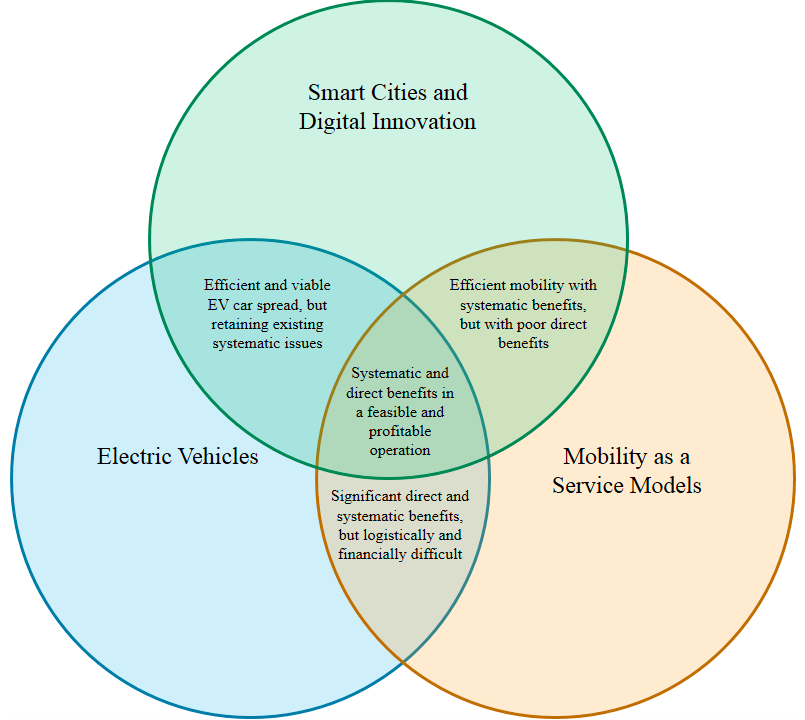
\includegraphics[width=0.6\columnwidth]{images/triopt.png}
\caption{The proposed `tri-opt' of positive opportunities to disrupt
  the private sector transport paradigm in developed countries.}
\label{fig:triopt}
\end{figure}

% old caption:
% Areas of double overlap correspond to a perception of the strengths
% and weaknesses in these combinations, as presented in the literature
% reviewed; the area of triple overlap is the stated hypothesis for this
% research.

\subsection{Electric Vehicles}

Electric vehicles (EVs), driven by electric motors powered by a
battery, have emerged as an environmentally sustainable alternative to
ICEs. As well as reducing carbon emissions, EVs typically have lower
noise and air pollution, can be cheaper to run per mile and reduce
transport's dependency on fossil fuels~\citep{postevs:2010}. It is
widely accepted that an alternate (and scalable) energy source is
necessary for the UK transport network in the future, with
electrification considered the most likely choice. Furthermore, the UK
Government's aspiration is that by 2040 every new car in the UK will
be an ultra low emission vehicle (ULEV): it is facilitating this
through a range of measures including financial support to help
consumers meet the upfront purchase costs of ULEVs, through a
``Plug-in Car Grant'' scheme, and investment in the creation of a
national charge point network~\citep{brook:2015}.

Most of the world's major automotive manufacturers have released
purpose-designed electric cars (different from ICEs that have a
substituted EV powertrain). Some have gone so far as to make
significant strategic investment in the concept by releasing entire
electric car ranges, such as BMW's i Series. Personal cars and small
commercial vehicles account for 13\% of all UK carbon
emissions~\citep{lumsden:2012} so the direct `pump-to-tire' benefits
of electric cars are highly significant. Legislation in many countries
is double-edged: penalising ICE users and incentivising the
purchase of EVs. EVs bring with them several challenges, however: the
purchase price of EVs, predominantly due to current battery
technology, is yet to be comparable to an equivalent ICE; the embodied
carbon of EVs, again due to the battery component, is typically higher
than an equivalent ICE; and the generation of electricity to meet
charging patterns is theorised to bring with it considerable
logistical difficulties on national
grids~\citep{su-et-al:2011,akhavan-rezai-et-al:2015}. Furthermore,
some of the benefits, such as CO$_2$ savings, are dependant on the
method of electricity generation used in the EV.

There are several barriers to the adoption of EVs; some of these are
psychological for the end user. ICE owners have shown range anxiety --
a concern over `running out of
juice'~\citep{oflev:2011,yilmaz+krein:2012}. Evidence rarely supports
such concerns: 95\% of all private vehicles journeys in the UK are
$<25$ miles~\citep{oflev:2011,brook:2015}, a distance current EVs are
easily able to service. Other user perceptions include concerns over
battery lifetimes, the risk of obsolescence from investing in a
product from a rapidly advancing technology, and the higher price of
EV purchase.  Many also criticise an absence of second-hand EVs for
purchase. Fleet vehicles accounted for 63\% of all new vehicle sales
in the UK in 2011; as such they are a dominant influence on the cars
that are subsequently available for sale in the secondary purchase
markets~\citep{fleets:2012}. There is a growing trend for EVs in fleet
vehicles due to reduced running costs, so it is likely a more
substantial used EV market will start to emerge in the near future.


\subsection{Digital Innovation and Smart Technologies}

`Smart' as a mechanism is a contemporary and rapidly growing area of
research and development (R\&D); as such, a consensus on the concept's
definition has yet to be established. A review of the academic, policy
and industrial practitioner literature in the field suggests a
recurring fundamental theme is the use of increased data (in volume,
quality and scope) and connectivity to create
value~\citep{komninos:2002,arup-et-al:2011,harrison+abbottdonnelly:2011,batty-et-al:2012,buscher:2014}. The
rise of interest in data-based value creation within cities can be
related to a number of trends:

\begin{enumerate}[i)]
\item {\emph{The rapid acceleration in the production of data.}}
Several key societal developments, including the rise of wide-spread
internet connectivity (particularly high-speed mobile connectivity)
and social networking, has caused an exponential increase in data
production; rapidly growing datasets have spurred experimentation as
to their potential new uses. `Big data' is regularly used to refer to
data available in such volumes, and is sometimes defined as a dataset
big enough to be considered for use in smart value-producing
systems~\citep{ojo-et-al:2015,sta:2017,mckinseysmartcities:2018}.
\item {\emph{The rapid increase in the ability to collect more
specific, higher-value data.}} Improvements in sensor and transmission
technology have resulted in data collection devices becoming more
financially affordable and spatially
practical~\citep{townsend:2013}. The development of mesh networks, the
mechanism of two-way communicating sensor nodes distributed over vast
areas, can provide high resolution data facilitating accurate
statements or the ability to reliably track and understand sensed
activity. Furthermore, the internet of things (IoT) -- defined as
two-way connectivity integrated into everyday items -- could enable
transitions from machine-human-machine interaction to simply
machine-machine.
\item {\emph{Improvements in data storage and processing.}} Storing
and processing data is becoming significantly cheaper, increasingly
based in the cloud. This enables complex, intensive analytics on vast
datasets -- such as on the scale of a city -- to be processed and
presented for actioning fast enough to be deemed `live'.
\end{enumerate}

Discussions increasingly refer to data as a raw material (sometimes
going so far as to describe it as an emerging fifth `utility'),
creating the notion that data can and should be used as a primary
input to a business model~\citep{arup-et-al:2011}. This may involve
aggregating or integrating data across traditional
`silos'~\citep{shapiro:2006,tsoukalas:2008}. Increasingly, this also
represents the pressing focus on whole-life environmental impacts of
ICTs~\citep{cooper-et-al-gsict:2015}. `Creating value' can be defined
in many ways, for example:

\begin{itemize}
\item {\emph{Faster processes:}} for example, using traffic data to
pro-actively update signs in real-time, rather than the slow, reactive
methods by which traffic is informally advised against taking certain
routes.
\item {\emph{Fairer:}} for example, real-time demand-based tolls for
motorways, charging higher rates for peak travel times, or when air
quality is particularly poor in the city, and, conversely, lower rates
at off-peak times.
\item {\emph{At lower cost:}} for example, water pipes containing flow
sensors to identify the accurate location of leaks as they emerge,
rather than expensive and time-consuming excavations and visual
inspections~\citep{cosgrave-et-al:2014}.
\item {\emph{Without human interaction:}} For example, when a first
aid dispatch can be made at the detection of a heart attack in a
public space, rather than requiring on-lookers to assess the situation
and intervene. This can reduce the impact of human error, social
boundaries and subjective judgement, although there is a discussion to
be had of the shortcomings of overly objective assessment in
processes.
\end{itemize}

It is acknowledged that a wide variety of big data applications are
not without ethical and societal
concerns~\citep{bimber:1990,metcalf-et-al:2016} -- especially raising
questions about civil liberties, privacy, mass surveillance and data
retention~\citep{goold:2002,oatley-et-al_dasc:2015,tryfonas-etal-has2016},
as well as wider concerns regarding technology dependency (perceived
or real), and the skills needed for effective societal
participation~\citep{tryfonas+crick:petra2018}.

However, there is an extensive literature documenting the potential
impact of digital innovation, through these improvements, in the
transport sector~\citep{enoch:2015}. One trend absent from the current
analysis is the issue of autonomous vehicles: if it were to be
included it might be considered within this category or as a separate
macro trend. While future extensions of this framework should seek to
incorporate this consideration, it is out of scope for this paper.

\subsection{New Ownership Models}

`Mobility-as-a-Service' has grown to be a concept that is specifically
recognised in modern transport dialogues~\citep{tscatapult:2016}. It
is best defined as a transition from a paradigm under which mobility
functionality is accessed through purchasing a product, to a paradigm
where mobility functionality is the outcome of a service moving users
from one location to another, disassociated from any requirement for
asset ownership, and typically arranged on a journey-by-journey basis.

In other modes of private transport in the UK, such as bike use, an
increasing number of citizens are participating in short term hire
models of use, particularly in urban contexts. Rather than bearing the
capital and logistical cost of owning a bike, individuals rent the
bike from a node near the origin of their journey, complete their
journey, and return the bike to a node near their destination. As such
they are purchasing the outcome of mobility from one destination to
another, or `as-a-service'. Once seen as radical, examples such as
London's cycle hire scheme, or the spread of ride hailing services
such as Uber and Lyft, have demonstrated not only the popularity of
the operating model, but also the indirect benefits (for example,
illustrated by the significant increase in cycling in the city,
bringing wider health benefits). A range of drivers have been
suggested for the emergence of this paradigm:

\begin{itemize}
\item {\emph{Changing societal values:}} evidence has
suggested a decrease in the cultural value placed on car ownership;
conflict with an increased desire to live in vibrant urban areas
within walking distance of workplace and other amenities and the
spatial restrictions of car ownership in such
scenarios~\citep{jenks+burgess:2011}.
\item {\emph{Changing economic situations:}} increasing costs of car
ownership, particularly in insurance (particularly for young
individuals) and fuel cost.
\item {\emph{Changing effectiveness of privately-owned car
transportation:}} an increasing frustration with congested transport
systems and an increasing desire to travel A-to-B reliably,
regardless of the specific comfort of one's `own' motor vehicle.
\item {\emph{Proof of concept:}} Driven by commercial ventures showing
the viability of alternate private transport paradigms. Traditional
car hire companies in particular are beginning to explore short-term,
distributed `car club', return journey (`A-to-A' journeys) offerings,
whereas emerging start-ups are offering complete A-B services, such as
the aforementioned Autolib.
\end{itemize}

% \subsection{The UK Context}

% In the UK, over the last 60 years, the profile of citizen journeys has
% transitioned rapidly from public transport dominated to private
% transport-dominated, stabilising around the last millennia
% [FOOTNOTE1]. Vocal, anti-automotive political agendas, global
% recession and rising oil prices have all emerged since as powerful,
% anti-private transport influences. However, they have done little to
% reduce private transport, with the per-mile travel profile appearing
% largely unchanged, tending instead to a marginally lower equilibrium
% level from 2000 to today. This is displayed in Figure 1a,
% contextualised by the historical car ownership trends in Figure
% 1b. However, there is emerging evidence that over the last 10 years,
% cars per person are declining, driven by lower ownership rates,
% particularly driven by younger drivers [REF6]. 


% \begin{figure}[!htp]
% \centering
% 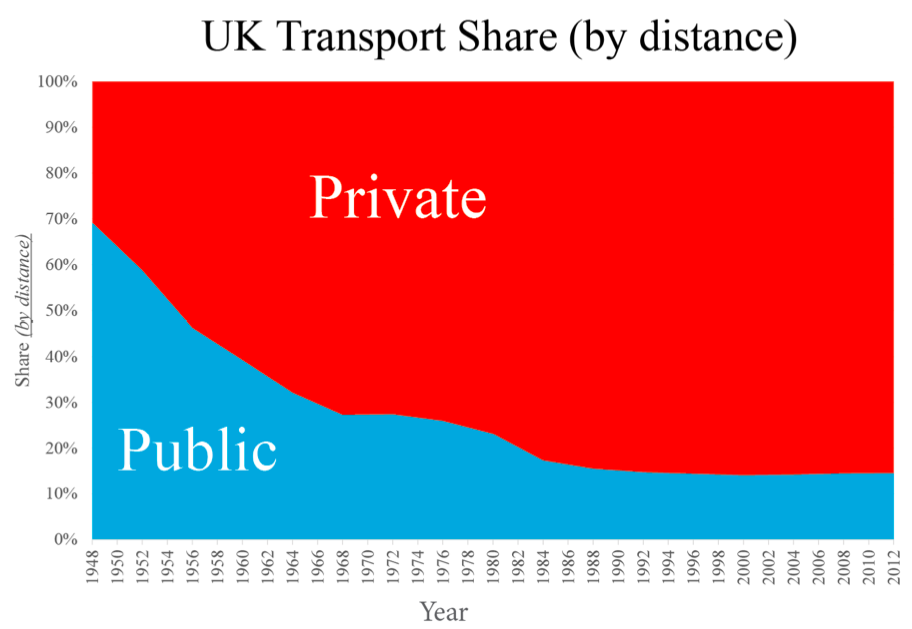
\includegraphics[width=\columnwidth]{images/uktransportshare.png}
% \caption{Car ownership trends in the UK}
% \label{fig:uktransportshare}
% \end{figure}

% \begin{figure}[!htp]
% \centering
% 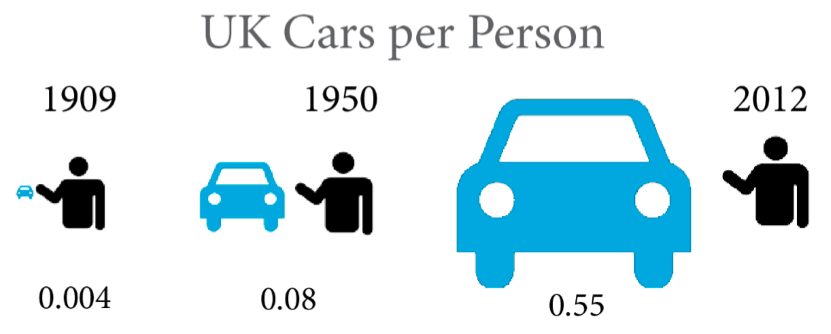
\includegraphics[width=\columnwidth]{images/ukcarsperperson.png}
% \caption{Transport share in the UK}
% \label{fig:ukcarsperperson}
% \end{figure}

% In theory, it is clear that at present public transport is both
% technically (in terms of emissions per head) and systematically
% (second-order effects, such as congestion, social and economic
% consequences) superior to private transport and this has been
% understood for some time [REF7]. However, it is equally apparent that
% the unit cost of converting a percentage of transport users from
% private to public transport increases with conversion. In other words,
% in a hypothetical world where everyone uses private transport, to
% convert the easiest first 10\% of users, a network of urban buses and
% trains can be run cost-effectively and efficiently. The last 10\% of
% the population, however, requires a vast and complex network that
% operates constantly and at high frequencies, and is for all intents
% and purposes, impossible to deliver. As such, it is clear that there
% is a fraction of transport that, for reasons of financial and
% practical limitations, will always remain private transport, and that
% that fraction is not necessarily `small'. Although the UK does not
% currently operate at or even near this ‘minimum’ private transport
% threshold, acknowledgement that any such unavoidable level exists is
% not necessarily popular in transport policy.

% As such, there is clear motivation that the impacts of private
% transport, both pump-to-tire and systematically, should be
% mitigated. This is a popular and high-growth area of research both
% commercially and academically; within the last 20 years, the average
% personal automobile efficiency has improved drastically.  Today,
% alternate  powertrains  such as electric motors that are more
% efficient and less polluting that ICEs, are not
% only technically viable, but a key component of many automotive giants
% strategies; the aforementioned BMW i Series range is a high profile
% example of significant strategic investment in the transition of
% retail automobiles to EVs. However, it is clear that drivetrain
% transitions alone cannot deal with the systematic drawbacks of private
% transport, such as congestion, spatial requirements of parking and
% social isolation of the have-cars and have-nots, which have been
% addressed to an order-of-magnitude lesser extent. Technical
% suggestions for these problems do exist, such as driverless, automated
% cars and personal rapid transit (PRT) schemes, but both are a long way
% from a ready-to-rollout status [REF8]. Crucially, for every change
% that reduces the negative impact of private transport (of either
% kind), or more accurately, convincingly depicts itself as doing so,
% private transport is further legitimised, and efforts to transfer
% journeys to public transport are weakened. Thus improvements to the
% performance of private transport need to be sufficiently substantial
% to mitigate any systematic `rebound' effect of reduced public
% transport use.
 
% Private transport solutions are almost exclusively the remit of the
% private sector; if we focus on the mode of car, these can be broadly
% categorised as automotive retailers, car hire firms and taxi
% companies. The public sector’s potential influence is relatively broad
% and classifiable into two main groups. Firstly, regulation, subsidies
% and taxation, which while exercised to bring about sustainability
% improvements in car design and car use, are generally applied at an
% industry level and are balanced against other political desires such
% as keeping motor product prices low and the automotive commercial
% environment favorable to investment [REF9]. Secondly, through the
% provision of infrastructure, which while said to be becoming
% increasingly mindful of its systematic impacts, is still predominantly
% designed to meet the current and near-future needs of its users rather
% than dictate them (Institution of Civil Engineers, 2016). 

% Political action is thus limited by this simple catch-22: public
% transport is the ideal, but impractical to reach saturation. Private
% transport is undesirable, but unavoidable, yet efforts to improve it
% also make it more prevalent. Private transport services must remain
% commercially profitable if they remain in the hands of the private
% sector, and at present, the government appears not inclined to lead
% radical changes in its nature from the limited influences it has at
% its disposal. It seems change must come primarily from the private
% sector (Westlake, 2016).

% Technically, it may be argued there thus exists an optimum – a level
% of improvement of private transport that, when the reduction in public
% transport uptake is factored in, results in the lowest overall impact
% in the UK’s travel emissions. There are many more secondary effects
% that could also be considered from this first deduction; not all
% improvements to private transport reduce public transport uptake to
% the same degree; nor is the UK a homogenous mass of two types of
% transport user. Attempts to penalise private transporters who could
% transfer to public transport and do not, such as through taxation,
% frequently damages those who cannot transfer [REF10] [REF11].

We can see how the opportunities introduced come together to address
three of the main difficulties in the current transport paradigm in
the UK:

\begin{enumerate}
\item {\textbf{Electric vehicles:}} enabling significant improvement
in the direct, pump-to-tire impacts of private transport, one of the
most substantial steps toward long-term achievements in this space;
\item {\textbf{Digital innovation:}} enabling significant improvement
in operational cost, customer engagement, system management and new
revenue streams, addressing the private sector's requirement for
profitable ventures;
\item {\textbf{Mobility-as-a-Service:}} enabling significant
improvement in the systematic impacts of private transport, a radical
first step in achievement in this space.
\end{enumerate}

However, there are shortcomings of these new mobility forms, including
shifting workforce demands, rebound effects increasing car-based
mobility, as well as the challenges of promoting cycling for
transport~\citep{handy-et-al:2014}. The actions of transport
stakeholders in the next 10 years will dictate how much these trends
are harnessed, encouraged or ignored in private sector transport, and
ultimately how the UK's transport culture changes as a
result~\citep{rode-et-al:2017}.

\section{Methodology}\label{methodology}

\subsection{Objectives}

This paper thus sets out to achieve the following objectives:

\begin{enumerate}[i)]
\item To explore a range of use cases in the UK's private transport
system that involve the three elements of the `tri-opt'. These use
cases must use at least two of the three elements in combination and
produce value;
\item To understand, with a qualitative degree of accuracy, the varying
value perceived by stakeholders in the identified `combination' use
cases;
% \item To understand the broad characteristics of the identified use
% cases, with a focus on barriers and enablers to their valuation and
% implementation.
\item To segment the use cases, considering their characteristics,
value potential and value certainty, with a view to identifying
recommended actions for policymakers;
\item Finally, to explore and better understand the interaction of the
  three elements of the `tri-opt'.
\end{enumerate}

\subsection{Philosophy}

This paper adopts a systems-thinking perspective to consider instances
when these trends create double and triple overlaps. For discovered
instances, interaction of the `tri-opts' will be explored, the value
perceived in the use case identified, and certainty of that value
measured. With respect to the definition and measurement of value, due
the broad scope of this paper, value is considered qualitatively
through research facilitator review (detailed in the following
section), with an emphasis on comparative value: a use case's value
compared to that of other identified use cases. Value to all
stakeholders within the system boundary will be considered; in this
case the UK city of Bristol.

\subsection{Methods}

The research objectives imply a mixed methods approach. The work is
primarily -- but not exclusively -- based on a research study into the
potential of a `smart electric vehicle transport hub' -- a proposed
development that combined the three proposed trends on a physical site
offering both public (bus and `park and ride') and private
(as-a-service electric car hire) transport services -- see
Figure~\ref{fig:bristolhub}. The methods used are as follows:

\begin{itemize}
\item Five two-hour workshops involving Bristol City Council staff,
University of Bristol academics, and consulting engineers from a
multi-national built environment consultancy firm;
\item Ten semi-structured one hour interviews with a range of
transport stakeholders in the city of Bristol, including bus
operators, policymakers, legal and financial professionals. All
providing insight anonymously;
\item A survey of 48 citizens of Bristol subscribed to Source West, an
independent non-profit organisation representing the interests of
citizens using electric vehicles;
\item Systems modelling to better understand the perceived value in a
selection of specific use cases, explained in more detail when
introduced.
\end{itemize}

\begin{figure}[!hb]
\centering
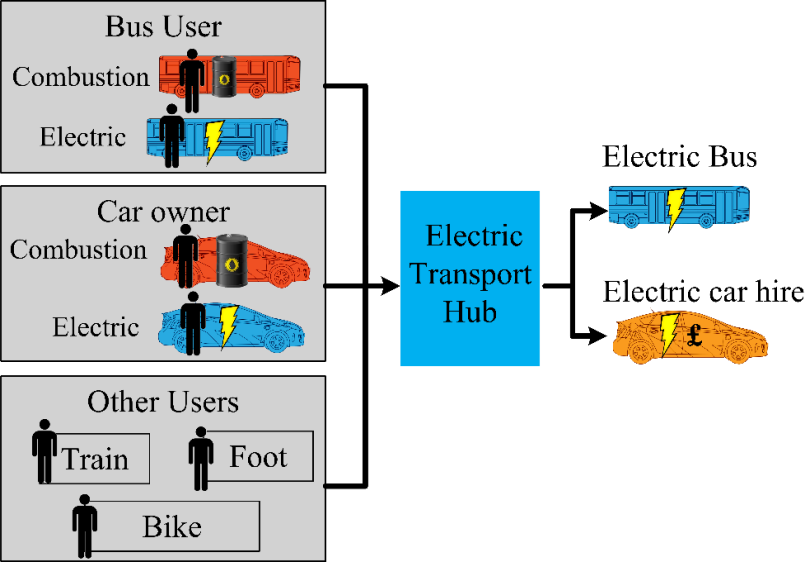
\includegraphics[width=0.75\columnwidth]{images/bristolhub.png}
\caption{An overview of the proposed Smart Electric
  Transport Hub, structured by input transport modes (left) and output
  transport services}
\label{fig:bristolhub}
\end{figure}

Throughout the first two components of the method, use cases that were
discovered, and the role of the `opts' within them, were
documented. The researchers scored participants' views and reactions
against two dimensions:

\begin{itemize}
\item {\emph{The value:}} Participants were encouraged to articulate their
perception of the scale of the benefit to all stakeholders within the
city. Researchers then estimated this sentiment using an approximate
scale of 0-100 where: 0 corresponded to no perceived value in any
circumstance; 50 a moderate but noteworthy value; and 100 a value of
substantial magnitude that could not conceivably be made meaningfully larger.
\item {\emph{The certainty:}} Participants were encouraged to articulate
their perception of the certainty of their value estimations. Researchers then
estimated this sentiment using an approximate scale of 0-100 where: 0
corresponded to stakeholders suggesting their estimation was
essentially random and dependent on a vast range of unpredictable
external factors; 50 indicated a relatively confident estimate but that was
reliant on some external factors; and 100 a technical certainty that
relied on no external factors.
\end{itemize}

The third and forth components of the method were used primarily to
shape and detail certain use cases, and did not directly feed into
scoring.\\

Individuals were selected for the workshop and interview based on four
criteria: 

\begin{itemize}
\item Individuals involved in the delivery of services in
the UK city of Bristol who have a deep understanding of
the performance criteria of these systems and what value may look like
from the operator perspective;
\item Individuals who have experience of the urban challenges of the
city and have a strong understand of what value looks like from a
public good perspective;
\item Individuals who had expertise in MaaS, EV and smart
transport solutions in private transport systems in the UK;
\item Individuals who those in the previous three groups recommended for
insight on the problem space.
\end{itemize}

\subsubsection{Workshops}

Prospective candidates with the highest scores across the four
criteria above were prioritised as workshop participants rather than
interviewees. The workshops were iterative, designed to build a use
case library while refining understanding of value and value
certainty. The other methods proceeded in parallel. As such, workshop
participants were -- as much as practical -- constant throughout.
Each workshop was structured in the following manner: presentation of
identified use cases so far; open discussion of possible new use cases
or new segmentation of existing use cases; discussion of evidence on
perceived value and value certainty in use cases, based on data
provided and participant viewpoints. The workshops were designed so
that all participants were able to contribute to all use cases.

\subsubsection{Interviews}

Interview participants were recruited using the same method as
workshop participants. The interviews were all semi-structured and
following best practice guidance from ~\citet{king+horrocks:2010}. All
interviews followed the same broad structure: participant background
(e.g. the individual's experience and their current role), broad
discussion of the problem space and alignment around issues (i.e. the
`tri-opt' as a concept and its component parts); an exploration of how
these concepts might create use cases and their benefits, providing
space both to propose new use cases and also to test on-going
hypotheses; finishing with a free discussion.

\subsubsection{Assessment}

Interviews were manually coded using Computer-Assisted Qualitative
Data Analysis Software (CAQDAS). Coding was used to find commonalities
across suggested use cases; comments regarding value and value
certainty; and comments regarding the wider context and about barriers
and enablers. The process of quantifying qualitative information was
based on the 8-step process~\citep{chi:1997}. In particular, Chi's
recommendation to increase reliability by using multiple raters was
implemented.

% results
\section{Value Cases for EVs-as-a-Service in Bristol, UK}

% \subsection{Overview}

% The results are presented in the following format:

% \begin{itemize}
% \item {\emph{Individual Use Cases:}} A profile of each individual
% use cases identified as a result of the methodology, articulated as
% communally defined by stakeholders participating. Each use case is
% labeled with the relevant `Opts' they involve;
% \item {\emph{Use Case Value Comparison:}} A value map of the use
% cases, as described in Section~\ref{methodology};
% \item {\emph{Individual Barrier and Enablers:}} A profile of each of
% the identified barriers and enablers, identified as a result of the
% methodology, articulated as communally defined by stakeholders
% participating. On review of the results, the cross-applicability of
% these makes it logically to present these as a communal set. However
% particularly strong applicability of one barrier/enabler to a
% particular use case will be emphasised in that barrier/enabler's
% description.
% \end{itemize}

%\subsection{Individual Uses Cases}

\subsection{Car Component State (Smart/MaaS/EV)}

In the traditional car hire industry, it is common practice to run a
maintenance program that involves inspection at a greater frequency
than that recommended for a privately-owned automobile, designed to
reduce the likelihood the car might suffer from a failure while hired
by a customer.

Using mechanical health sensors -- that could be considered a `smart'
element -- attached to key components in the car an operator offering
cars-as-a-service could gather insight on a car's mechanical state
close to the quality of that offered by a human inspection, in real
time. This has the potential to reduce the rate of failures in such a
service. If the sensor coverage were sufficient then this could lead
to cost savings through reduced servicing and also decrease
turn-around times, important in a service that will have more frequent
car hiring than a traditional arrangement. This servicing issue is a
wider concern in an EV context, because the workings of EV
powertrains have less of a mechanical history than their ICE
counterparts simply because they are a more recent technology.

% AM: I'm not sure that 'exacerbated' is the right word here, and I'm
% not quite clear what the 'this' is that is being exacerbated. Is it
% the need for close monitoring? Or the difficulty of anticipating
% faults? Or the potential savings gain from a different type of
% monitoring?

\subsection{Live Air Quality Management (Smart/MaaS)}

Bristol City Council currently monitors air quality through a
portfolio of permanent and semi-permanent sensor installations at
points distributed around the city. In a typical UK urban environment,
particularly one with no major heavy industry, air quality is
primarily determined by road transport emissions, particularly those
of diesel vehicles~\citep{bbcnews:2017,glaaqd:2018}. It can be
hypothesised that if it was possible to understand the distribution of
vehicles in the city at any one point in time, combined with other
factors such as weather, it would be possible to estimate the air
quality across the entire city, to an acceptable degree of accuracy.

At present, in certain areas of Bristol, car flow is monitored by
automatic number plate recognition (ANPR) cameras. Coverage is,
however, limited and scaling this infrastructure can be prohibitively
expensive. Cars-as-a-service vehicles are likely to have
near-identical behaviour to other cars on the road at that time. With
sufficient coverage of hire cars distributed among the main car park,
the total car distribution in Bristol could be extrapolated. Today
other datasets exist for understanding car movements around a city
(for example, Google Maps), but this is not always available to city
managers, nor is it necessarily free. This information could be
complemented by data from air quality sensors directly affixed to
cars.

%We will examine critical resolutions in detail in Section~\ref{barriersenablers}.


\subsection{Live Accident Reporting (Smart/MaaS)}

Cars could be fitted with impact sensors, alerting a cars-as-a-service
monitoring system that a car has suffered a crash, enabling them to
immediately alert the authorities. A number of trends have
significantly improved road safety in the UK over the last 20
years~\citep{dftsafetystats:2018}; combined with the relative rarity
of users of this type of monitoring system, the impact on rural
isolated crashes has not resulted in tangible improvement in injury or
fatality rates. Instead, it is more likely that the main benefit of
such a system would be an improved perception of safety by the
user. It may also be possible that through connectivity to city
transport systems, a system could alert traffic control teams of
potential disruptions.

\subsection{User Journey Data (Smart/MaaS)}

Social media websites have shown that advertisement hit rates can be
improved by accurate targeting of the advert to the correct
recipient. Depending on the medium of transport being used,
historically this technique would be attempted by advertising at a
particular time or in a particular geographical area. Today, however,
consumers are increasingly expressing preferences and specifics
relating to their personal situation through various social media
networks. It is thus possible to target individuals on a range of
highly specific criteria, such as a relationship status, group
affiliation or patrons of specific rival businesses.  Facebook and
Spotify are frequently highlighted examples of how these mechanisms
can not only deliver high conversion rates -- enabling the advertising
to be sold at higher prices -- but also enable the sale of smaller,
but still effective, advertising packages to smaller businesses. This
mechanism could produce value in a cars-as-a-service offering in two
identified ways.

Information on the journeys of car hire users, contextualised with
time of use and demographic details, could be sold -- wider privacy
and ethical considerations notwithstanding -- as data valuable to
companies in local retail and leisure sectors. Such clients can
consider the expensive customer research they would otherwise have to
undertake to obtain such data, and so a base price is conceivable.
Alternatively, such data could be used in-house in the form of
targeted advertising in-vehicle. Organisations could partner with the
service, offering promotional deals to users it believes it may be
able to induce to patronise their business during or after the
trip. This could be done in real-time using spatial data e.g. when the
vehicle occupied by the individual approaches a particular
business. The value creation could be twofold: the advertising
organisations could pay for the in-car advertising rights if they are
simply showing promotional material; if appealing deals were
exclusively available in-car then the take up of the cars-as-a-service
offer could increase. This second mechanism is likely to enjoy higher
data consent rates from users because the value to them is more
direct.


\subsection{Demand-based Pricing (Smart/MaaS/EV)}

An alternate method to control congestion is to bring economic forces
to bear on individual travel choices. In practice, the pricing of MaaS
could incorporate an additional influence based on the expected
congestion of the roads at point of travel, attempting to deter travel
that would exacerbate congestion. Ultimately, of all the use cases
addressed here this requires the highest critical resolution of a MaaS
service. Furthermore, many ethical dilemmas exist. It might be
extremely unpopular that the most sustainable cars are essentially
`taxed' into staying off the roads, while unsustainable private
transport isn't obliged to bear the cost of the externality it is
generating.

An alternative, and more common, reason for using dynamic pricing is
around the ability to better control demand for the service. This is a
key consideration for electric vehicles due to the fact that, even
with the increasing affordability of fast chargers, EVs require
considerably longer than ICE cars to transition from zero to full
range capacity.

Finally, dynamic pricing could also be used to manage car supply and
demand between different nodes of car collection. There are a number
of scenarios where the ability to maintain a serviceable fleet at a
node could be jeopardised:

\begin{enumerate}
\item {\emph{Inclement driving conditions:}} Compared to ICEs, EV's
energy consumption per mile is more susceptible to influence from
weather conditions. Colder weather can have negative effects on the
motor and battery performance. Furthermore, car cabin heaters in EVs
do not have engine heat stream to redirect, so additional power from
the battery is required to generate this, measured to be as much as
15\%~\citep{dft:2008,brook:2015}. Live battery data could enable the
cars-as-as-service management system to know the exact power use of a
journey and thus the expected battery use available at the end of a
journey.
\item {\emph{Congestion:}} High levels of traffic, resulting in
`stop-start driving', can significantly decrease the efficiency of an
EV, although the effect is not as pronounced as with an ICE because an EV
powertrain can turn off and on, thereby conserving energy. Congestion also
increases journey time. Car speed data and GPS location data could
inform the booking management system when a car is likely to have
reduced efficiency, and when it is unlikely to be back at a node when
expected.
\item {\emph{Satellite navigation:}} Knowing the intended destination
of a user can help pre-empt different levels of EV occupancy at nodes,
and advise where a space needs to be made available. Furthermore, live
satellite navigation data can advise what route is taken, and how this
effects the arrival time and level of charge at arrival.
\end{enumerate}

Pre-warning of any of these unforeseen circumstances can allow
immediate shifting of the booking system to reflect increased hire
duration or increased charging duration. This will prevent people
booking in a time when the car will now be driving/charging. This
system delivers value through the improved reliability of the car hire
service. Insight from these and other scenarios will advise the
cars-as-a-service operation system of when which specific EVs are
likely to be at which nodes and with what charge, allowing
interventions that adjust pricing at different nodes to ensure space
at current destination nodes and availability of charged cars across
all nodes.

An example of a simple dynamic pricing formula can be seen in
Figure~\ref{fig:smartpricingformula} whereby the size of the `smart
power' constant determines the influence of the dynamic component.
Simulations based on such an algorithm were used to explore the
potential impact of demand-based pricing on revenue and variance of
booking density for a designed service of `smart EV MaaS'. The results
are presented in Figure~\ref{fig:smartpricegraphs}.


\begin{figure}[!ht]
\centering
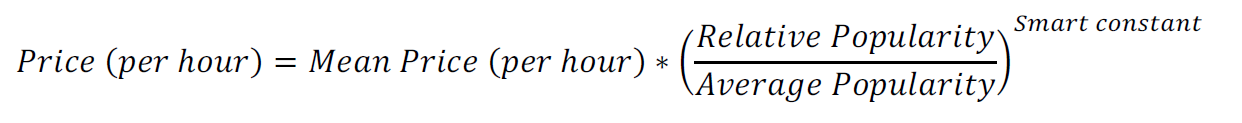
\includegraphics[width=0.75\columnwidth]{images/smartpricingformula.png}
\caption{Smart pricing formula}
\label{fig:smartpricingformula}
\end{figure}

% \begin{figure*}[htb]
% \centering
% 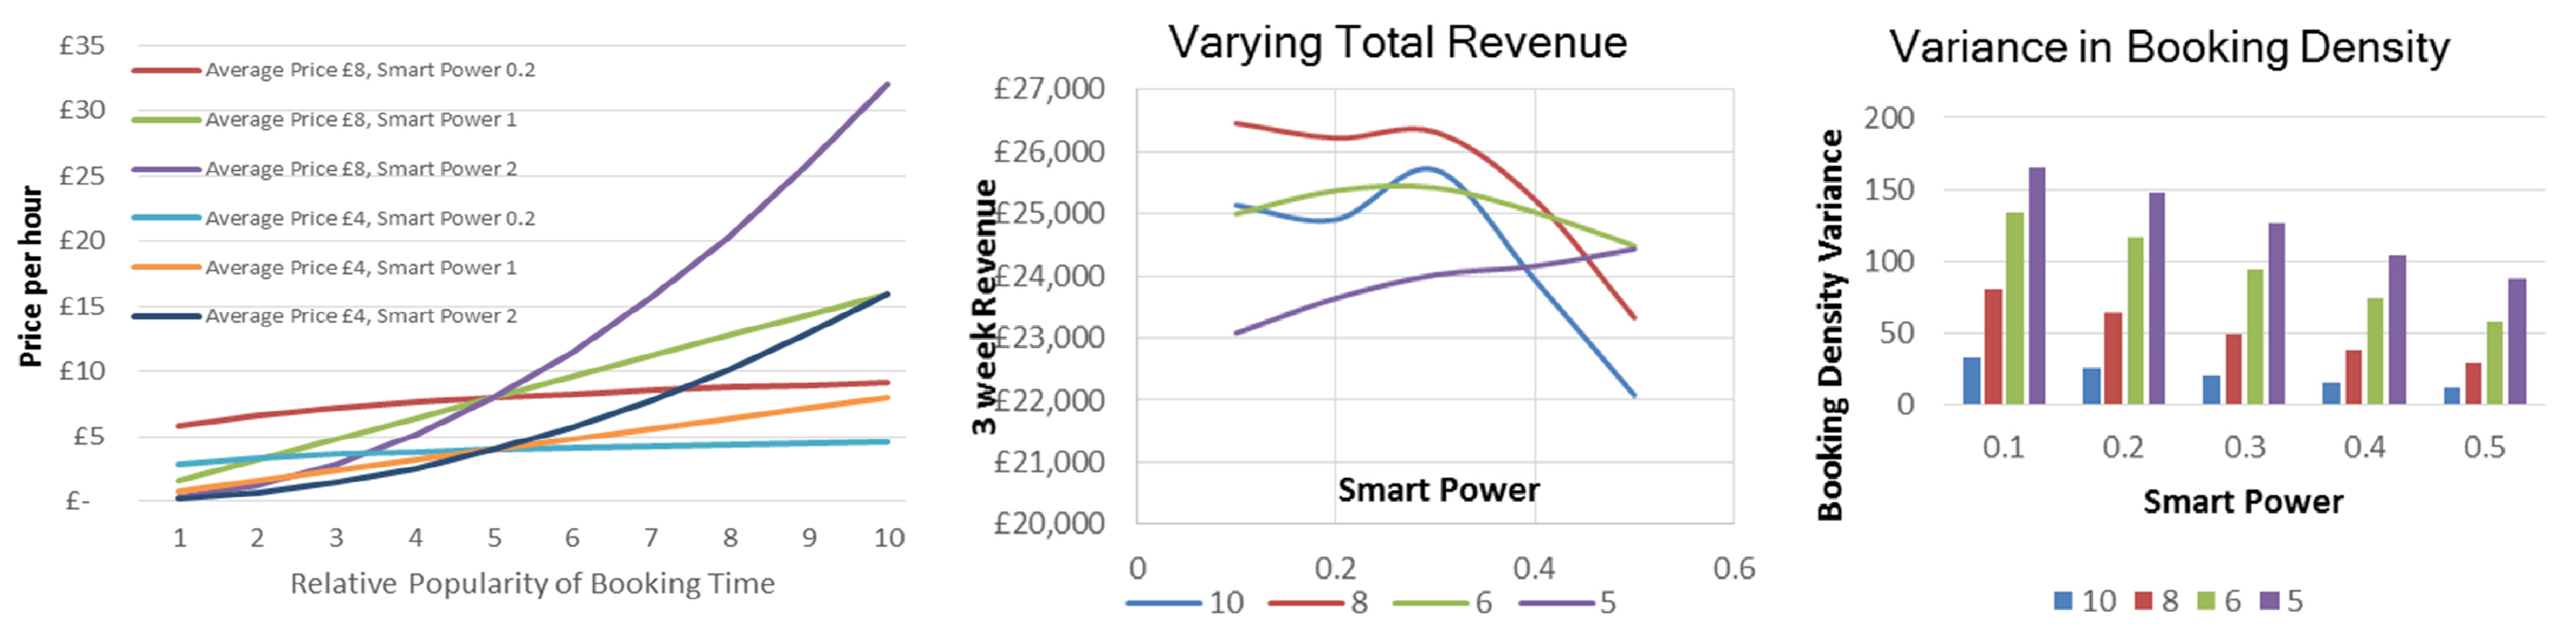
\includegraphics[width=\textwidth]{images/smartpricegraphs.png}
% \caption{Data regarding varying dynamic pricing rates (left) derived
% from Figure~\ref{fig:smartpricingformula} and their effect on revenues
% (centre) and booking densities (right). Collected during the
% {\emph{Bristol Smart EV Hub}} project.}
% \label{fig:smartpricegraphs}
% \end{figure*}

\begin{figure}
\centering
\begin{subfigure}[b]{0.6\textwidth}
  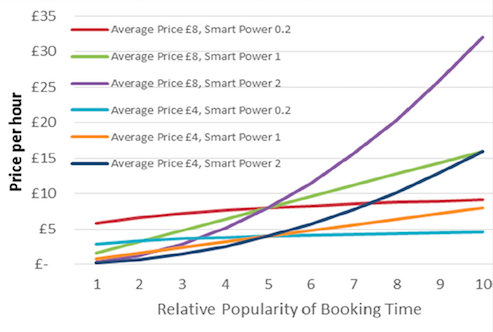
\includegraphics[width=\textwidth]{images/smartpricegraph1.png}
        \caption{}
        \label{fig:smartpricingrates}
\end{subfigure}

\begin{subfigure}[b]{0.6\textwidth}
  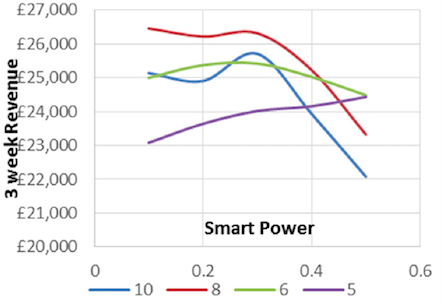
\includegraphics[width=\textwidth]{images/smartpricegraph2.png}
        \caption{}
        \label{fig:smartrevenues}
\end{subfigure}

\begin{subfigure}[b]{0.6\textwidth}
  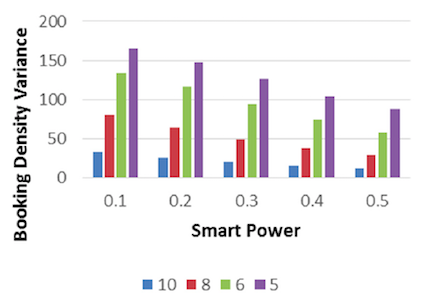
\includegraphics[width=\textwidth]{images/smartpricegraph3.png}
        \caption{}
        \label{fig:smartbookingdensities}
\end{subfigure}
\caption{Data regarding varying dynamic pricing rates (a) derived
from the smart pricing formula in
Figure~\ref{fig:smartpricingformula}, and their effect on revenues
(b) and booking densities (c).}
\label{fig:smartpricegraphs}
\end{figure}

% old caption:
% From left to right: Price ranges with different formula values;
% Varying total revenue under different schemes; Variance in booking
% density, a measure of the difficult of servicing bookings, with
% different ‘smart powers’ and average prices. Draws on data regarding
% price sensitivity, customer flexibility and estimated footfall
% collected during the Bristol Smart EV Hub project.

On certain theoretical assumptions about customer behaviour,
it is possible to create a scenario through dynamic pricing where both
total revenue is increased and bookings are more evenly
distributed. This mechanism could be made stronger, or seen to be more
of a `carrot' than a `stick' strategy, by using reduced parking costs
in non- or limited-nodal MaaS systems.

\subsection{Driving Styles and Usage Habits (Smart/EV/MaaS)} 

As a high growth market, the EV market is currently undergoing heavy
R\&D investment. As a distinctly different driving experience,
automotive designers are particularly interested in how users interact
with the vehicle~\citep{ferreira-et-al:2013}. Such data is not
commonplace and, therefore, to create an evidence base car
manufacturers spend capital on customer surveys, on-road testing and
other investments.

A similar situation can be observed in the car insurance industry:
while the total cost of ownership of hybrid and electric vehicles
compared to conventional vehicles has reduced from the year of
introduction~\cite{palmer-et-al:2018}, at present relatively few car
insurers offer cover for EVs due to a poor understanding of their
risk. Those who do offer insurance price it at an average of 16-26\%
above the ICE equivalent. It is unclear if EV owners drive in an
identical manner to combustion car owners, or if they are at a higher
risk of collision due to lower noise and potential driving profiles
than ICE cars. Furthermore, many fundamental components of the EV have
yet to come close to their expected end of life, so it is risky for
insurers who do not know if the vehicles will reach their rated life.

The UK's National Grid could derive value from understanding how EV
charging in a cars-as-a-service model has an impact on the grid,
steering their strategic investment accordingly.  Although information
is available around how privately-owned EVs require
charging~\citep{kennel-et-al:2012,darabi+ferdowsi:2013}, EVs making
frequent trips throughout the day could have distinctly different
charging requirements. The value of this insight also extends to
regional distribution network operators: they hold the responsibility
for ensuring local networks can service supply, upon which the nodal
distribution of MaaS cars could have significant impacts. It is
reasonable to assume these datasets also have a value to the operator
of an EV MaaS system, through external sale, if an appropriate data
strategy were in place.

\subsection{Dynamic Traffic Routing (Smart/MaaS)} 

Understanding the average speed of a road's cars allows the city's
transport management to predict areas of congestion. The data
resolution needed for this is much lower i.e. the speed of a given
stretch of road is largely similar for all vehicles driving along
it. A city transport management team with access to such information
in real-time can employ data-based traffic management techniques. One
of the most common such technique is dynamic traffic re-routing. Road
users are directed to the fastest route to a given location by being
mindful of congestion. The car hire scheme takes this concept one step
further, as it will be possible to understand where individuals are
planning on driving in advance. With this information, mitigation
actions that would previously be considered to have too long a lead
time even in the 'live' mode can be implemented. For example, higher
use of contraflow lanes that can be dynamically adjusted to allow for
the particular nature of rush hour traffic, increased public
transport frequencies to help move demand off the roads, or variable
speed limits to maximise flow rates and relieve bottlenecks.

Much of the infrastructure necessary to facilitate this has already
been tested at scale: dynamic lane direction has proven successful on
the M6 (intercity) motorway around Birmingham and the M25 London
orbital motorway in the UK, with extensive supporting evidence about
its dynamic speed limit interventions. The effectiveness of this
infrastructure could be improved by using data that arrive faster and
more accurately than generated by existing, predominantly analogue,
sensing techniques.  A criticism of this concept might be that such
datasets are currently collected by global technology firms such as
Google. Such data however is not readily available to cities and, when
it is, it typically comes with a substantial cost. A MaaS service
would be an alternative route to accessing this data and could provide
it to the city's transport team.

\subsection{Grid Balancing (EV/Smart/MaaS)} 

Grid balancing is a generalised term for the concept of taking action
to mitigate against substantial divergence between supply and demand
in regional or national electricity systems. In some definitions,
balancing involves transferring power into the grid, but many
techniques of simply avoiding drawing power (a.k.a. {\emph{shaving}})
or moving the demand to another period (a.k.a. {\emph{shifting}}) are
considered balancing by the UK Government~\citep{decc:2014}. The
challenge of balancing the network is becoming much larger as a
consequence of more distributed generation and larger power
demands. Many stakeholders in the UK's energy industry are
increasingly providing financial incentives for these services and
view it as an important challenge of the future. Almost all of these
solutions involve some aspect of a `smart grid', i.e. that data is
used in the management of these interventions.

This difficulty is highly relevant to EVs because they represent a
growing load on the grid; some studies have suggested even moderate
uptake of EVs might increase national power demand by up to 23\% in
some areas by 2021~\citep{paffumi-et-al:2015}. However, of greater
concern is that EVs will increase the variation
(essentially the peakiness) in demand, a quality that is harder for
the grid to service than total demand. However, at the same time the
potential of EVs to be used as charge storing devices enables a
situation whereby, theoretically, rather than being seen as a burden
on the grid which needs to be minimised, they could be seen as a
positive asset to provide charge to meet demand at peak
times. Typically batteries have a very quick response rate to grid
requirements, something other balancing solutions can lack.

In a MaaS offering, the value of the charge to the grid at a
particular time could be factored in to the cost of someone hiring the
car, and so using the charge instead to drive the car. This would
enable more opportunities for charge to be provided for grid balancing
at times of need. Logistically, a MaaS arrangement would have EVs
plugged in by default (requiring no manual intervention as likely with
privately-owned EVs). Furthermore, such systems would also typically
have large numbers of EVs connected to the grid on connections with
substantial voltage capacity, facilitating sudden charge and discharge
actions.

This potential for considering MaaS EVs as an asset to the grid comes
with the caveat that required charging for the cars' actual purpose
can be sufficiently shifted to be of negligible impact. This is
compounded by the context that many of the business models around
balancing systems have yet to achieve commercial viability, and may
not develop in the UK for at least 10 years. This, along with the
general penetration of EVs -- MaaS or otherwise -- is an important
factor to consider for this use case, but it is not relevant to our
primary focus of examining the overlaps associated with the `tri-opt'.

% \section{Barriers and Enablers}\label{barriersenablers}

% \subsection{Overview}

% Throughout the workshop and interview process it became apparent that
% there were substantial barriers to both the realisation of these use
% cases, and barriers to being more certain about the specific value
% they could bring. On balance, there were also certain common enablers,
% which added clarity to these two aspects.  This section profiles those
% that were communally considered to be the most important across all
% use cases.

% \subsection{Devolution}

% In the UK devolution is a defining trend of local governance. Cities
% are increasingly being given more power and more responsibility to
% fund and deliver many of their own services. Combined with a landscape
% of fiscal austerity, this combines to provide the motivation, and
% capability, to experiment with new solutions that can deliver better
% outcomes on a smaller budget, or that drive growth, sustainably,
% growing the overall city purse. Driving potential new transport
% initiatives, such as the use cases explored herein, could be such an
% action.

% \subsection{Legislation}

% At present legislation around EVs is rapidly evolving. Only recently
% in the UK it became legal to charge for electricity partiers who
% weren’t registered electricity supplier. Up until this point, although
% designed to enforce strict license requirements, restrict `cowboy'
% generators and limit electricity theft, the law greatly prohibited the
% ability to charge for electrical charging for EVs. 

% Furthermore, subsidies are a high risk reliance. Payouts for balancing
% services are complicated and have questionable longevity.  There is
% little immediate governmental impetus for demand-based energy pricing
% to support the Grid Balancing use case. However, many energy companies
% have begun distributing smart meters, which many have suggested is the
% best precursor to new demand-based tariffs.

% \subsection{Perception}

% Despite considerable feature in literature, conference and
% international economics as a whole, the value of smart technologies as
% a concept has yet to be universally realised by the business world as
% a whole. Many surveys have suggested that concepts such as Big Data
% analytics remain the domain of large corporations, and are sometimes
% viewed with risk and pessimism by many smaller, regional
% firms. Although motivation for smart city approaches is high in local
% government, a lack of private-sector buy-in becomes a prohibitive
% barrier.  The legacy of many unexpanded `demonstrator' Smart City
% projects compounds this issue (Arqiva, 2015).

% \subsection{Citizen Culture Shock}

% The freedom to use a car when one desires is heavily ingrained in
% Western society, and it's likely some of the use cases examined
% herein, particularly those that involve changing the price of using a
% car when a large number of individuals want to use one, would receive
% significant citizen backlash and so become politically unpopular. The
% most effective implementation of these is likely to be focused around
% shaping these perceptions, such as ostensibly offering financial
% advantages for `good' behaviour, rather than exclusively penalising
% `negative' use. 

% \subsection{Critical Resolutions}

% The issue of critical resolution presents an issue particularly for
% the more macro concepts.  Modelling undertaken the Smart Electric
% Transport Hub project illustrates this barrier. Using the estimated
% number of cars in a rough 2x2 mile square of urban Bristol at peak
% time, Figure 16 demonstrates a simulation of the accuracy of the
% Dynamic Traffic Routing use case, given a varying distribution of
% connected, EV cars within the car parc. The accuracy is defined as the
% ability to state whether a 10 yard x 10 yard area of the city has an
% above average level of car presence.

% As per Figure~\ref{fig:criticalresolution}, the results are
% particularly interesting; at present private EV rates (around
% 0.001\%), the ability to perceive areas of congestion is abysmal,
% correctly identifying congestion vs no congestion with around 5\%
% accuracy. However, by 0.14\%, the system has surpassed the odds of
% simple guessing, and by 0.7\%, the system has reached an impressive
% 90\% accuracy. 0.7\% corresponds to around 70 cars; the quantity you
% might envisage within such a sized zone in a multisite implementation
% of a single MaaS node in Bristol. It is also worth noting that the
% assumptions here are particularly pessimistic -- if spots of higher
% density (rather than simply above average) wished to be found, the
% accuracy will theoretically improve.

% \begin{figure}[!htb]
% \centering
% 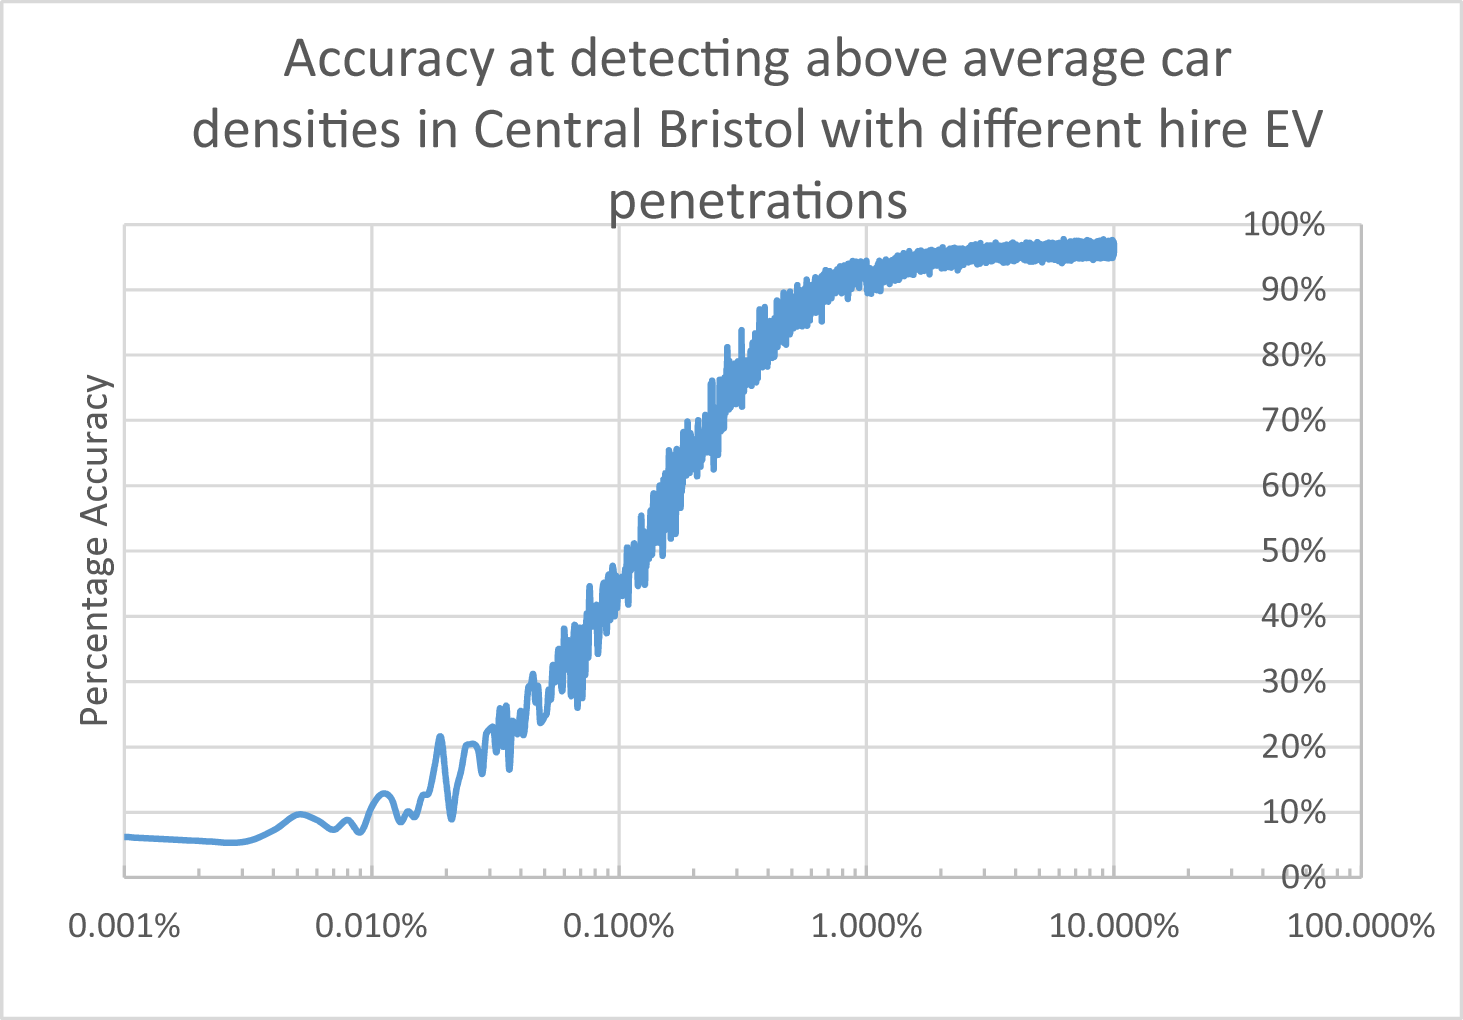
\includegraphics[width=\columnwidth]{images/criticalresolution.png}
% \caption{MATLAB modelling of the accuracy of extrapolating to find
%   congestion from connected EV cars in Bristol, UK}
% \label{fig:criticalresolution}
% \end{figure}

% \subsection{Collective Ownership of Functioning Cars Achieved Through
%   MaaS}

% It was identified that some of the concepts identified are considered
% significantly feasible as a result of the nature of the MaaS asset
% ownership. In theory, a car park of `smart' cars that were privately
% owned and ICE powertrain could be sufficient to facilitate,
% theoretically, some of the concepts, such as Dynamic Car
% Routing. However, MaaS is associated as a core aspect of these use
% cases because the centralised ownership of the cars means that
% connected cars can be immediately purchased, and the data is
% considered the operators to use as desired, pending user consent,
% which in turn would be a requirement for use of the MaaS service in
% any way. The concept based on privately-owned car ownership however,
% would take longer to implement as individual's cars are gradually
% replaced with more intelligent cars (assuming they make mainstream
% markets). This organic growth may encounter issues of interoperability
% between cars and systems. Regardless, citizens would need to be
% persuaded to provide their data, and it would not be a requirement for
% the use of the car for them to do so.


% \subsection{Need for Public-Private Collaboration}

% By far the most substantial barrier identified during workshops and
% interviews was the requirement for public and private sector
% stakeholders to collaborate to implement many of the use cases,
% particularly those perceived to have the greatest value. This barrier
% is perceived to have two key caveats:

% \begin{itemize}
% \item The distribution of value created for difference stakeholders is
%   not aligned with the risk and investment each stakeholder is making
%   – many of the concepts herein would create value for the city they
%   are operated in, such as through congestion reductions, air quality
%   improvement, economic growth, that would not translate, even over a
%   long timeline to financial returns for the private sector operator
%   of a smart EV MaaS service. However, the value to the city could be
%   traced to tangible reductions in spending in various other
%   initiatives. As such, business models need to be explored whereby
%   clarity on these distributed benefits is established, and
%   appropriate financial arrangements made to motivate the private
%   sector to push ahead with the investment.
% \item Different capabilities and cultures between the two stakeholder
%   groups – in the context of collaborating on a transport project, a
%   perception was raised that private sector companies are
%   traditionally focused on profit rather than wider societal benefit,
%   but able to efficiently deliver services, think entrepreneurially,
%   and understand and meet customer requirements. At the same time
%   there was a concession that public sector organisations are
%   traditionally more cautious and slower to embrace digital change,
%   but have a more holistic assessment of transport solution and
%   societal benefits. Several case studies were offered by participants
%   to articulate this, particularly the failure of the Kutsplus Demand
%   Responsive Bus system in Finland (Westlake, 2016). Recognition of
%   these differences and creating strategies that embrace the qualities
%   of both will be essential if implementations are to be successful. 
% \end{itemize}

\section{Value Case Comparison}\label{usecasecomp}

%\subsection{Workshops/Interviews}

It is clear there is significant variation in the perception of value
in the identified use cases, and the certainty with which we understand
this value and the path to realising; these are presented in
Figure~\ref{fig:valuegraph}. From observation of the results, three
categories can be generalised:

\begin{itemize}
\item {\emph{Segment 3}} comprises those use cases that have by far
the greatest perceived value, but are also the most
uncertain. Typically these have the highest critical masses and
require considerable, cross-sector stakeholder buy-in. However, their
potential value could be described as extreme. Discussion highlighted
how these use cases typically have the most diverse forms of value,
spanning environmental, social and economic value, beyond simply
financial benefits. While these use cases are highly unlikely to be
implemented immediately due to the substantial barriers they face,
their significant potential cannot be ignored.
\item {\emph{Segment 2}} captures use cases with moderate benefit and
a lower level of uncertainty than those in segment 1. These use cases
enjoy a good overall value/certainty ratio. These are typically
mechanisms that involve the collection, management and external
vending of data. The value of these use cases will depend on how legal
and contractual norms around data trading evolve. Cities, including
Bristol, have launched open data initiatives, where certain public
sector datasets are made freely available for reuse. There is an
ongoing debate about how data monetisation strategies, such as those
identified in our use cases, are compatible with city open data
ambitions.
\item {\emph{Segment 1}} covers use cases with relatively low
perceived value but relatively high certainty. This group are best
characterised as 'operational' changes, and as such require relatively
little collaboration across stakeholder groups.
\end{itemize}

\begin{figure}[!h]
\centering
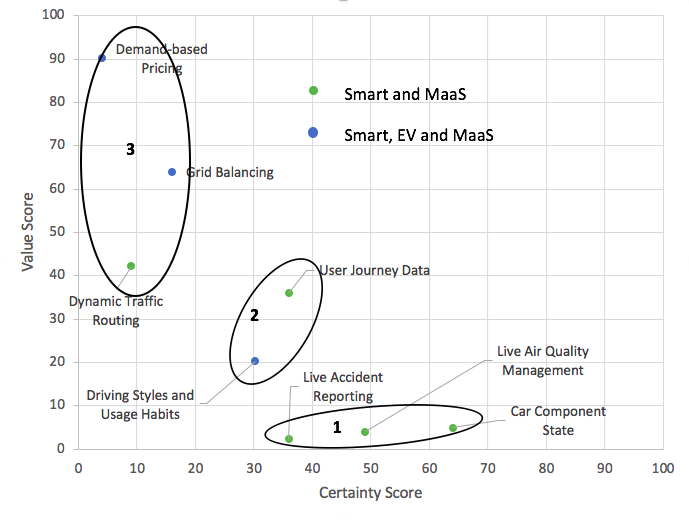
\includegraphics[width=0.75\columnwidth]{images/valuegraph.png}
\caption{Results from workshop exercises on assigning qualitative
value scores to use cases (note: log scale)}
\label{fig:valuegraph}
\end{figure}

Graphical approximations of these characteristics across the three
segments can be seen in Figure~\ref{fig:segmentcharacteristics}.

\begin{figure*}[!ht]
\centering
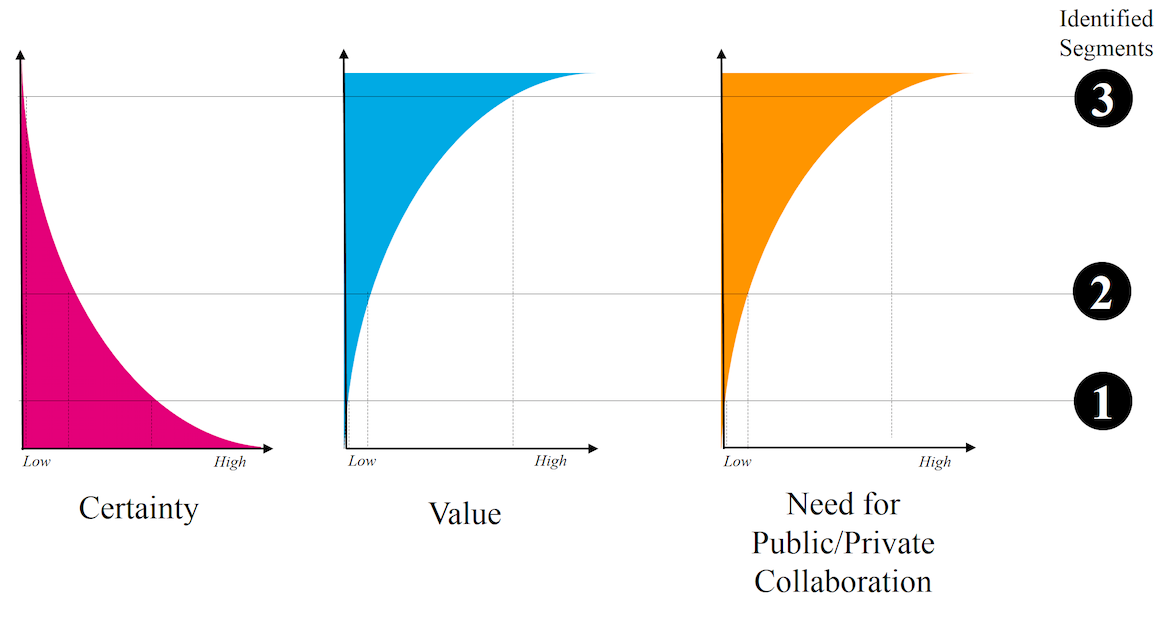
\includegraphics[width=0.8\textwidth]{images/segmentcharacteristics.png}
\caption{Generalised relationships across identified segments}
\label{fig:segmentcharacteristics}
\end{figure*}


% \subsection{Systems Dynamics}

% As a means of validation, these workshop findings have been compared
% to a systems dynamics model created to explore financial estimations
% of some of the identified concepts, per-node for the Hub
% project. While of a similar context, this model was created outside of
% this research initiative. A Sankey diagram out of this model can be
% seen in Figure~\ref{fig:sankey}.

% It can be observed that, allowing for small differences in the
% categorisation of use cases (some were dissected for easier
% modelling), definition of value and certainty, relative proportions
% match our workshop findings.
 
% \begin{figure}[!htb]
% \centering
% 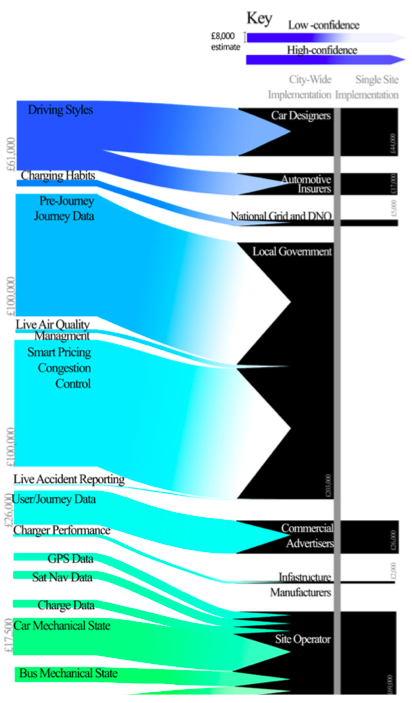
\includegraphics[width=\columnwidth]{images/sankey.png}
% \caption{Sankey diagram output of a systems dynamics model, exploring
%   the financial benefit of some of the identified use cases for a node
%   of the Hub.}
% \label{fig:sankey}
% \end{figure}


\section{Conclusions}\label{conclusion}

% AM: This conclusion is framed in terms of whether original hypotheses
% and speculations are confirmed or otherwise. Buy, maybe because of the
% editing for the revised version, I don't think the paper is now
% introduced by presenting those hypotheses/speculations.

There is clearly synergistic value within the overlaps of the proposed
`tri-opt'; however it appears the specifics of this are somewhat
different to initial speculation. The findings suggest use cases that
combine MaaS offerings and digital innovation are the main focus of
value creation, rather than those which seek to exploit MaaS, EV and
digital tri-overlaps. While we can still conclude that the triple
overlaps exist as an area to be considered, it may be better to
consider EVs as simply a `significant' development that is set within
the context of the two more transformative opportunities presented by
MaaS and digital innovation. Reviewing the concepts that have emerged
through our methodology, perceived value appears to take a wide range
of forms, but overall is significant. Certainty is also variable but
is generally scored at lower levels. This variability is to be
expected when considering that all the identified use cases represent
significant changes away from systems currently in operation, but are not
necessarily transformative in nature.

With respect to recommendations that can be inferred from these findings:

\begin{itemize}
\item {\emph{Segment 1}} should be considered good operational
practice for smart, MaaS EV services. However, they are not
transformative, and generally provide limited value, so might not
justify being treated as high priority.
\item {\emph{Segment 2}} should be considered as positive additional
revenue streams for smart, MaaS EV services. In particular, they may
be beneficial for improving business cases to the degree that such
services can attract investment and be launched, so releasing the
individual benefits of each ``Opt''. While offering good value for
relative certainty, they are not transformative in and of themselves.
As end goals they might be considered to lack ambition.
\item {\emph{Segment 3}} can be considered as the potential focus of
long term strategic planning that has transformative value, and have
underlying mechanisms that span beyond transport. Currently highly
uncertain, understanding these use cases, conceptually, should be a
high priority, cross-sectoral aspiration.
\end{itemize}

It is important to note that this paper does not set out to define the
value cases of the individual ``Opts'' themselves -- such as reducing
sunk-cost-induced car use in a MaaS model. It is designed to be a
study of interaction between the three broad developments, rather than
appraisal of each in isolation: there is extensive literature already
in existence addressing these issues separately, as noted in
Section~\ref{intro}. These recommendations should, however, be
appreciated within the context of the benefits of MaaS, smart cities
and digital innovation, and electric vehicles considered separately.

Our results suggest that there are significantly more barriers than
enablers at play in these double and triple overlapping concepts. Of
most significance in the eyes of the participants, and of most
relevance to the highest-value segment of use cases, is the need for
public and private sector collaboration. It seems reasonable to
presume this is a barrier for `as-a-service' and digital innovation
concepts across a range of city services beyond transportation.

\section{Future Work}\label{future}

For application beyond transport, it is recommended that the
underlying generic value creation mechanisms at play are further
explored. The particular emphasis on MaaS and digital innovation
suggests `digitally-enabled innovative business models' may be the
best starting point for the analysis. Taking away the transport
context, mechanisms observed included sharing of data to mutual
benefit (e.g. driving habits); supporting new service delivery models
that bring public benefit (e.g. dynamic car routing); and assistance
in delivering public policy (e.g. demand-based pricing to reduce
congestion). The mechanisms rest upon meaningful cross-sector,
public-private collaboration.

\begin{figure}[!h]
\centering
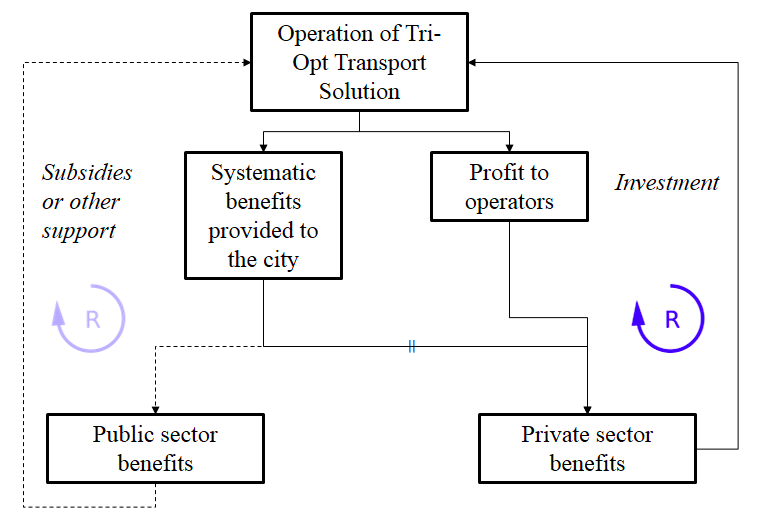
\includegraphics[width=0.7\columnwidth]{images/causalloop.png}
\caption{A causal loop diagram presenting the investment/value
  dilemma of certain `tri-opt' transport solutions.}
\label{fig:causalloop}
\end{figure}

Little or no research could be found that sets out a consistent
framework for representing and analysing these mechanisms. There is a
significant evidence base that private sector participation in city
digital initiatives is regularly criticised by the public
sector~\citep{martin:2016}. Yet, our work indicates that there is
value in understanding this issue better. Furthermore,
digitally-enabled public and private collaboration needs to be
understood better: our research highlights its absence as the major
current barrier to innovating to realise value. The distribution of
value/risk/investment identified as part of this, and articulated in a
simplified causal loop diagram in Figure~\ref{fig:causalloop}, needs
to be further investigated.

% acknowledgments
\section*{Acknowledgments}

This work was supported by the UK EPSRC-funded Industrial Doctorate
Centre in Systems (Grant EP/G037353/1) at the University of Bristol
and Arup Group Ltd. We would also like to acknowledge the support of
Bristol City Council and Source West for their involvement in the
project.

% references section
\bibliographystyle{abbrvnat}
\bibliography{jut2017}

% that's all folks
\end{document}


